\begin{figure}[t]
  \centering
  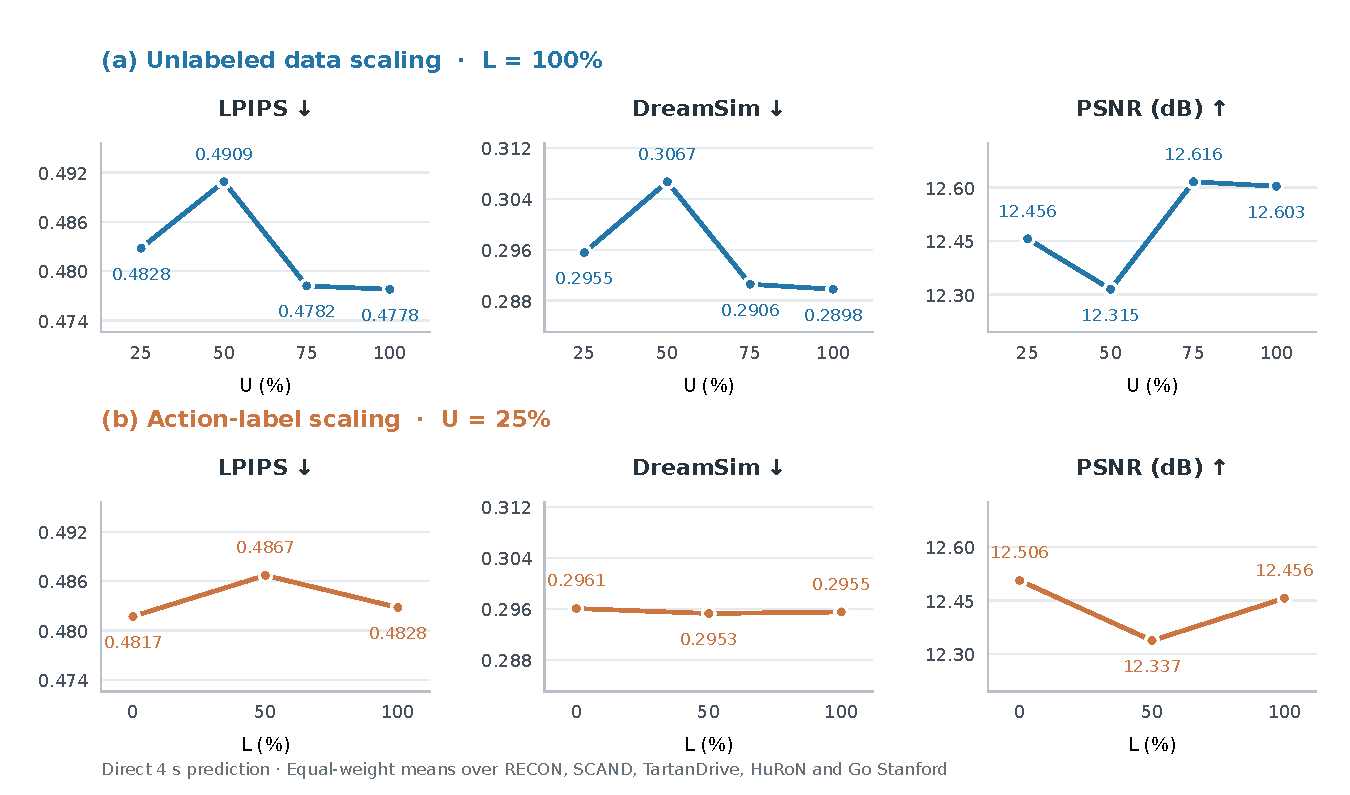
\includegraphics[width=\linewidth]{figures/data_scaling/data_scaling_mean_three_metrics.pdf}
  \caption{\textbf{Effect of data scaling on direct 4\,s prediction.}
  Top: unlabeled-data fraction $U$ varies with action-label availability
  fixed at $L=100\%$.
  Bottom: action-label availability $L$ varies at $U=25\%$.
  Columns show LPIPS, DreamSim, and PSNR, each averaged with equal weight
  over RECON, SCAND, TartanDrive, HuRoN, and Go Stanford.
  Lower LPIPS and DreamSim and higher PSNR indicate better performance.
  Vertical limits are shared within each column.
  All intermediate settings are shown: these mean metrics do not improve
  monotonically with either scaling axis.
  Each setting uses a single checkpoint and evaluation seed;
  lines connect measurements without fitting a scaling law.}
  \label{fig:data_scaling_mean_three_metrics}
\end{figure}
